Windows kan terwijl jij erop werkt data over de status van je systeem naar Microsoft sturen. Op basis van deze data kan Microsoft adviezen uitbrengen over je systeem.

Hier moet je goed over nadenken. Hoeveel data over je systeem, de applicaties die je gebruikt en de sites die je bezoekt wil je met Microsoft delen in ruil voor goede adviezen over hoe je je systeem beter kunt beheren en fine-tunen.

Om je te laten zien waar je kan instellen wat je met Microsoft deelt en wat dat voor consequenties heeft. Starten we de Settings app op, gaan naar System en dan naar Troubleshoot. Hier kunnen we bij opties bepalen of automatische troubleshooters mogen draaien. De keuze bij de opties zijn:
\begin{itemize}
\item Run automatically, don't notify me
\item Run automatically, then notify me
\item Ask me before running (default)
\item Don't run any
\end{itemize}

\begin{minipage}[t]{\linewidth}
\raggedright
\adjustbox{valign=t}{%
	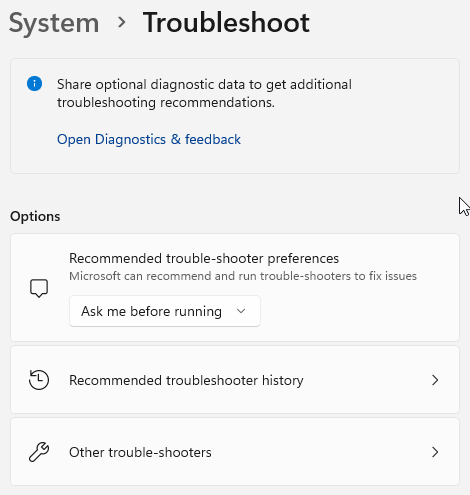
\includegraphics[width=0.99\linewidth]{settings_troubleshoot.png}%
}
\end{minipage}

Klikken we op \textquote{Open Diagnostics \& feedback} dan krijgen we nog veel meer opties die we kunnen instellen

\begin{minipage}[t]{\linewidth}
\raggedright
\adjustbox{valign=t}{%
	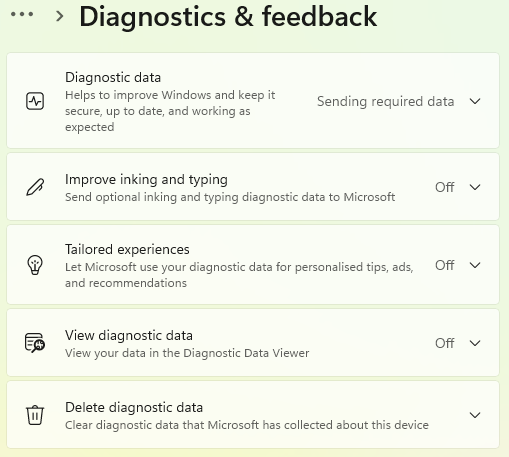
\includegraphics[width=0.99\linewidth]{settings-diagnostics_feedback.png}%
}
\end{minipage}

Loop door de verschillende items heen en kijk welke opties je aan of juist uit wil zetten.

Als we terug gaan naar de vorige pagina van de Troubleshoot settings, dan zien we dat er ook nog een kopje is met \textquote{Other trouble-shooters}. Hier kunnen we per onderdeel van ons systeem met hulp krijgen bij het onderzoeken van problemen met ons systeem.

